
\documentclass[12pt,a4paper,oneside]{report}

% -------------------------------------------------
% Packages and page layout (college project-report style)
% -------------------------------------------------
\usepackage[a4paper,left=1.25in,right=1.0in,top=1.0in,bottom=1.0in]{geometry}
\usepackage[T1]{fontenc}
\usepackage{newtxtext,newtxmath}
\usepackage{setspace}
\usepackage{graphicx}
\usepackage{float}
\usepackage{array}
\usepackage{longtable}
\usepackage{booktabs}
\usepackage{multirow}
\usepackage{tabularx}
\usepackage{enumitem}
\usepackage{titlesec}
\usepackage{tocloft}
\usepackage{fancyhdr}
\usepackage{hyperref}
\usepackage{xcolor}
\usepackage{tikz}
\usepackage{caption}
\usepackage{listings}
\usetikzlibrary{arrows.meta,positioning,shapes.geometric,fit,calc}

\definecolor{mgmpurple}{RGB}{76,20,125}
\definecolor{lightpurple}{RGB}{239,229,248}
\definecolor{lightblue}{RGB}{225,238,250}
\definecolor{lightgreen}{RGB}{225,243,229}
\definecolor{lightorange}{RGB}{255,239,218}

\hypersetup{
  colorlinks=true,
  linkcolor=black,
  urlcolor=blue,
  citecolor=black,
  pdftitle={Django Notes App Project Report},
  pdfauthor={Shrusti Chandole, Sanyukta Gandewar, Aarti Sangewar}
}
\onehalfspacing
\setlength{\parindent}{0.35in}
\setlength{\parskip}{3pt}
\renewcommand{\arraystretch}{1.25}
\setcounter{secnumdepth}{3}
\setcounter{tocdepth}{2}

\titleformat{\chapter}[display]
  {\normalfont\bfseries\centering}
  {\chaptername\ \thechapter}{8pt}{\Large\MakeUppercase}
\titlespacing*{\chapter}{0pt}{-15pt}{24pt}
\titleformat{\section}{\normalfont\bfseries}{\thesection}{0.8em}{}
\titleformat{\subsection}{\normalfont\bfseries}{\thesubsection}{0.8em}{}

\pagestyle{fancy}
\fancyhf{}
\fancyhead[C]{MGM'S COLLEGE OF ENGINEERING, NANDED}
\fancyfoot[C]{\thepage}
\renewcommand{\headrulewidth}{0.4pt}
\renewcommand{\footrulewidth}{0pt}

\lstset{
  basicstyle=\ttfamily\small,
  breaklines=true,
  frame=single,
  columns=fullflexible,
  showstringspaces=false
}

\begin{document}

% -------------------------------------------------
% TITLE PAGE
% -------------------------------------------------
\begin{titlepage}
\thispagestyle{empty}
\begin{center}
\vspace*{0.45in}
{\Large\bfseries A PROJECT REPORT ON}\\[0.35in]
{\Huge\bfseries\color{mgmpurple} DJANGO NOTES APP}\\[0.18in]
{\large A Dockerized Web-Based Notes Management Application}\\[0.55in]

Submitted to\\[0.12in]
{\large\bfseries DR. BABASAHEB AMBEDKAR TECHNOLOGICAL UNIVERSITY, LONERE}\\[0.25in]
in partial fulfilment of the requirements for the degree of\\[0.2in]
{\Large\bfseries BACHELOR OF TECHNOLOGY}\\[0.08in]
in\\[0.08in]
{\large\bfseries COMPUTER SCIENCE \& ENGINEERING}\\[0.45in]

{\large\bfseries By}\\[0.15in]
{\large Shrusti Chandole}\\
{\large Sanyukta Gandewar}\\
{\large Aarti Sangewar}\\[0.4in]

Under the Guidance of\\[0.12in]
{\large\bfseries Dr. S. Y. Gaikwad}\\[0.45in]

{\bfseries DEPARTMENT OF COMPUTER SCIENCE \& ENGINEERING}\\
{\bfseries MAHATMA GANDHI MISSION'S COLLEGE OF ENGINEERING}\\
{\bfseries NANDED (M.S.)}\\[0.2in]
{\bfseries Academic Year 2026--2027}
\end{center}
\end{titlepage}

% -------------------------------------------------
% CERTIFICATE
% -------------------------------------------------
\pagenumbering{roman}
\chapter*{Certificate}
\addcontentsline{toc}{chapter}{Certificate}
\begin{center}
\textbf{This is to certify that the project entitled}\\[0.2in]
\textbf{\large ``Django Notes App''}\\[0.2in]
submitted by\\[0.1in]
\textbf{Shrusti Chandole}\\
\textbf{Sanyukta Gandewar}\\
\textbf{Aarti Sangewar}\\[0.2in]
to the Dr. Babasaheb Ambedkar Technological University, Lonere, for the award of the degree of Bachelor of Technology in Computer Science and Engineering, is a record of project work carried out by the students under my supervision and guidance. The matter contained in this report has not been submitted to any other university or institute for the award of any degree.\\[0.45in]
\end{center}

\vspace{0.5in}
\noindent
\begin{tabularx}{\textwidth}{X X}
\centering\textbf{Dr. S. Y. Gaikwad}\\
\centering Project Guide
&
\centering\textbf{Head of Department}\\
\centering Computer Science \& Engineering
\end{tabularx}

\vspace{0.8in}
\begin{center}
\textbf{Director}\\
MGM's College of Engineering, Nanded
\end{center}

% -------------------------------------------------
% ACKNOWLEDGEMENT
% -------------------------------------------------
\clearpage
\chapter*{Acknowledgement}
\addcontentsline{toc}{chapter}{Acknowledgement}
We express our sincere gratitude to our project guide, Dr. S. Y. Gaikwad, for the valuable guidance, continuous support and encouragement throughout the study and preparation of this project. The suggestions and discussions helped us understand the design of a Django web application and the practical aspects of containerized deployment.

We also take this opportunity to thank the Head of the Department of Computer Science and Engineering for academic support and for providing the opportunity to undertake this project. We are grateful to the Director and the management of Mahatma Gandhi Mission's College of Engineering, Nanded, for providing the facilities and learning environment required for project work.

We acknowledge the developers and maintainers of the open-source technologies used in this project, including Python, Django, Docker, Docker Compose, MySQL, Nginx, Gunicorn and Jenkins. Their documentation and community resources were useful in understanding the implementation and deployment configuration.

Last but not least, we extend our sincere thanks to our classmates, friends and family members who directly or indirectly supported us during the completion of this work.

\vspace{0.35in}
\begin{flushright}
With sincere regards,\\[0.15in]
Shrusti Chandole\\
Sanyukta Gandewar\\
Aarti Sangewar\\
B.Tech. Computer Science and Engineering
\end{flushright}

% -------------------------------------------------
% ABSTRACT
% -------------------------------------------------
\clearpage
\chapter*{Abstract}
\addcontentsline{toc}{chapter}{Abstract}
The Django Notes App is a web-based application intended to provide a convenient digital space for creating and managing personal notes. The project uses the Django web framework and demonstrates how a Python web application can be packaged and deployed through Docker. The repository contains the Django application source code, a Dockerfile, a Docker Compose configuration, Nginx configuration, a MySQL service definition and a Jenkins pipeline file.

The deployment configuration defines three principal services: a Django application service, a MySQL database service and an Nginx web server. Docker Compose coordinates these services and connects them through a shared application network. The Django service applies database migrations and starts the application through Gunicorn. MySQL stores application data using a mounted data directory, while Nginx acts as the web-facing entry point. Health-check commands are configured for the database and Django service to help identify service readiness.

The repository also includes a Jenkinsfile describing pipeline stages for retrieving source code, building a Docker image, publishing the image to Docker Hub and invoking a deployment step through a shared Jenkins library. This project therefore provides a practical introduction to web application development and DevOps concepts such as containerization, service orchestration, reverse proxying, persistent storage and continuous integration/deployment.

This report presents the background, objectives, system modelling, requirements, methodology, implementation details, testing approach, results, limitations and future scope of the Django Notes App. The technical description is based on the publicly supplied repository and its visible configuration. Actual user-interface behaviour and deployment results should be verified against the final running application before academic submission.

\vspace{0.1in}
\noindent\textbf{Keywords:} Django, Python, Notes Management, Docker, Docker Compose, MySQL, Nginx, Gunicorn, Jenkins, Containerization, DevOps, CI/CD.

% -------------------------------------------------
% CONTENTS
% -------------------------------------------------
\clearpage
\tableofcontents
\clearpage
\listoffigures
\clearpage
\listoftables

% -------------------------------------------------
% CHAPTER 1
% -------------------------------------------------
\clearpage
\pagenumbering{arabic}
\chapter{Introduction}

Digital note-taking has become an important part of academic and professional work. Students regularly record lecture points, organise ideas, prepare revision material and retrieve information. Paper notebooks are useful, but they can be difficult to search, back up and access from different devices. A web-based notes application offers a convenient alternative by allowing information to be stored and accessed through a browser.

The Django Notes App is a Python-based web application built using the Django framework. The supplied repository also demonstrates how the application can be packaged into a Docker image and operated as part of a multi-service environment. The deployment configuration includes Django, MySQL and Nginx services coordinated through Docker Compose. Gunicorn is used as the WSGI application server for Django, and a Jenkinsfile describes an automated build-and-deploy pipeline.

\section{Background}
Django is a high-level Python web framework that provides URL routing, request handling, template rendering, an object-relational mapper and an administrative interface. These facilities make it suitable for building data-driven applications. A notes application typically receives a request from a browser, validates the submitted information, performs database operations and returns an updated page.

Containerization addresses differences between development and deployment environments. A Docker image packages application code and runtime dependencies. A container runs the image in an isolated process environment. Docker Compose describes related services in a YAML file so that they can be created and managed together.

\section{Problem Statement}
A notes application must provide a dependable way to store and retrieve user-created information. Deploying a web application directly on a host machine may require manual installation and configuration of the runtime, database and web server. Differences between machines can lead to dependency conflicts or inconsistent behaviour. The problem addressed by this project is to provide a Django-based notes application and demonstrate a repeatable containerized deployment setup in which the web application, database and reverse-proxy services are configured and operated together.

\section{Project Objectives}
The main objectives of the project are:
\begin{itemize}[leftmargin=0.4in]
\item To study and understand the structure of a Django-based notes application.
\item To package the Python application and its dependencies using a Dockerfile.
\item To coordinate the application, database and web server using Docker Compose.
\item To configure MySQL as the database service and provide persistent storage.
\item To use Gunicorn to serve the Django WSGI application.
\item To configure Nginx as the web-facing reverse proxy.
\item To understand service dependencies, health checks, networking and container lifecycle management.
\item To study the Jenkins pipeline stages for source retrieval, image build, publishing and deployment.
\end{itemize}

\section{Features and Functionality}
The repository and deployment configuration indicate the following project components:
\begin{itemize}[leftmargin=0.4in]
\item Django application source for the notes management workflow.
\item A Python application image defined through a Dockerfile.
\item MySQL database service for relational data storage.
\item Nginx service as the HTTP entry point and reverse proxy.
\item Gunicorn process for serving the Django WSGI application.
\item Docker Compose configuration for multi-service deployment.
\item Persistent host storage for MySQL database files.
\item Health checks for the Django and MySQL services.
\item Jenkins pipeline definition for build, image publishing and deployment stages.
\end{itemize}
The exact note operations, user roles and interface features should be described using screenshots and a live demonstration of the final application.

\section{Technology Stack}
The project configuration uses Python 3.9 as the Docker base image, Django as the web framework, MySQL as the database, Docker and Docker Compose for containerization and orchestration, Nginx as the reverse proxy, Gunicorn as the WSGI server, and Jenkins for the pipeline definition. Git and GitHub are used for source-code management.

\section{Scope}
The scope includes the Django application repository, container build configuration, multi-service orchestration and the deployment pipeline description. It covers the interaction between the browser, Nginx, Django/Gunicorn and MySQL. It does not claim a production cloud deployment, HTTPS configuration or successful execution of the Jenkins pipeline unless these are demonstrated in the final environment.

% -------------------------------------------------
% CHAPTER 2
% -------------------------------------------------
\chapter{System Modeling}

\section{System Architecture}
The system is organised into three principal runtime services. The browser sends an HTTP request to Nginx. Nginx forwards the request to the Django application service. Django processes the request and communicates with MySQL when database access is required. Gunicorn serves the Django WSGI application.

\begin{figure}[H]
\centering
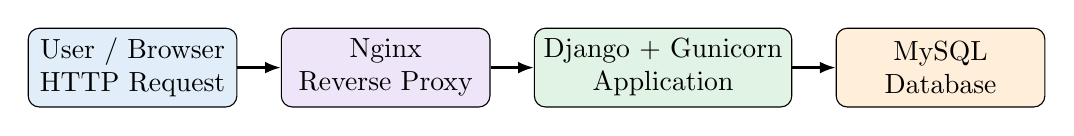
\begin{tikzpicture}[
 node distance=0.55cm,
 block/.style={draw,rounded corners,minimum width=2.65cm,minimum height=1.0cm,align=center,fill=lightblue},
 arr/.style={-{Latex[length=2mm]},thick}
]
\node[block] (user) {User / Browser\\HTTP Request};
\node[block,right=of user,fill=lightpurple] (nginx) {Nginx\\Reverse Proxy};
\node[block,right=of nginx,fill=lightgreen] (django) {Django + Gunicorn\\Application};
\node[block,right=of django,fill=lightorange] (mysql) {MySQL\\Database};
\draw[arr] (user)--(nginx);
\draw[arr] (nginx)--(django);
\draw[arr] (django)--(mysql);
\end{tikzpicture}
\caption{High-level system architecture}
\label{fig:architecture}
\end{figure}

\section{Data Flow Diagram}
The request processing sequence begins when a user opens the notes application in a browser. The browser sends an HTTP request to the host endpoint. Nginx receives the request and forwards it to the Django service. Gunicorn invokes the Django WSGI application. Django routes the request to the relevant view and performs the required application logic. If persistent data is required, Django connects to MySQL. The response is returned through Nginx to the browser.

\begin{figure}[H]
\centering
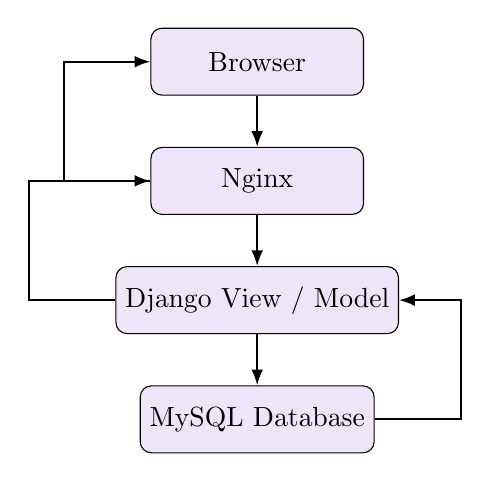
\begin{tikzpicture}[
 node distance=0.65cm,
 block/.style={draw,rounded corners,minimum width=2.7cm,minimum height=0.85cm,align=center,fill=lightpurple},
 arr/.style={-{Latex[length=2mm]},thick}
]
\node[block] (a) {Browser};
\node[block,below=of a] (b) {Nginx};
\node[block,below=of b] (c) {Django View / Model};
\node[block,below=of c] (d) {MySQL Database};
\draw[arr] (a)--(b);
\draw[arr] (b)--(c);
\draw[arr] (c)--(d);
\draw[arr] (d.east) -- ++(1.1,0) |- (c.east);
\draw[arr] (c.west) -- ++(-1.1,0) |- (b.west);
\draw[arr] (b.west) -- ++(-1.1,0) |- (a.west);
\end{tikzpicture}
\caption{Request processing and data flow}
\label{fig:dataflow}
\end{figure}

\section{Database Design Considerations}
The repository configures MySQL as a separate service and sets a database name through the container environment. Django models and migrations define the application database structure. The visible Compose configuration runs \texttt{python manage.py migrate --noinput} before launching Gunicorn, so pending schema migrations are applied at application startup.

A notes application commonly stores note content and related metadata as database records. The exact fields, relationships and constraints must be taken from the Django model definitions in the final source code. This report therefore describes the database at the service and persistence level rather than inventing unverified model fields.

\section{Deployment Architecture}
The Compose file declares a dedicated network named \texttt{notes-app-nw}. Nginx is built from the \texttt{./nginx} directory and publishes host port 80. Django is built from the project context, publishes port 8000, reads variables from \texttt{.env}, depends on the database service and uses a health-check endpoint. MySQL uses a host-mounted directory for its data files.

\begin{figure}[H]
\centering
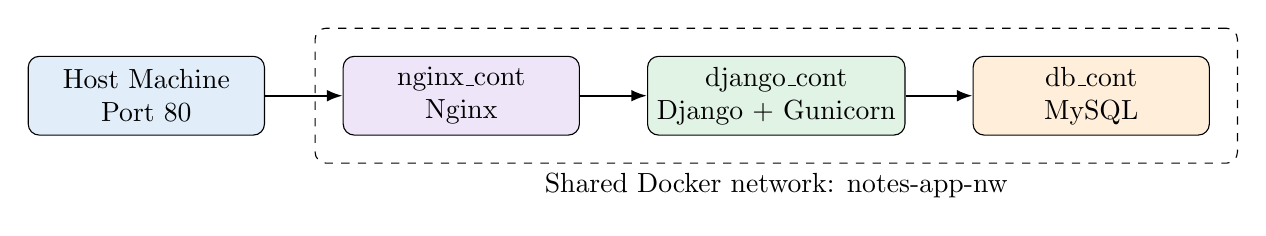
\begin{tikzpicture}[
 block/.style={draw,rounded corners,minimum width=3.0cm,minimum height=1.0cm,align=center,fill=lightblue},
 arr/.style={-{Latex[length=2mm]},thick}
]
\node[block] (host) at (0,0) {Host Machine\\Port 80};
\node[block,fill=lightpurple] (ng) at (4,0) {nginx\_cont\\Nginx};
\node[block,fill=lightgreen] (dj) at (8,0) {django\_cont\\Django + Gunicorn};
\node[block,fill=lightorange] (db) at (12,0) {db\_cont\\MySQL};
\draw[arr] (host)--(ng);
\draw[arr] (ng)--(dj);
\draw[arr] (dj)--(db);
\node[draw,dashed,rounded corners,fit=(ng)(dj)(db),inner sep=0.35cm,label=below:{Shared Docker network: notes-app-nw}] {};
\end{tikzpicture}
\caption{Docker Compose deployment architecture}
\label{fig:compose}
\end{figure}

\section{Main Repository Components}
\begin{longtable}{|p{0.30\textwidth}|p{0.60\textwidth}|}
\hline
\textbf{Path / File} & \textbf{Purpose}\\ \hline
\texttt{api/} & Application API-related source folder.\\ \hline
\texttt{mynotes/} & Notes application source folder.\\ \hline
\texttt{notesapp/} & Django project configuration package and WSGI entry point.\\ \hline
\texttt{nginx/} & Nginx build and reverse-proxy configuration.\\ \hline
\texttt{staticfiles/} & Static assets collected or served by the application.\\ \hline
\texttt{Dockerfile} & Defines the Python-based application image build.\\ \hline
\texttt{docker-compose.yml} & Defines Nginx, Django and MySQL services, networking and volumes.\\ \hline
\texttt{Jenkinsfile} & Describes the CI/CD pipeline stages.\\ \hline
\texttt{requirements.txt} & Lists Python package dependencies.\\ \hline
\texttt{manage.py} & Django command-line utility.\\ \hline
\texttt{.env} & Environment configuration file; real secrets should be protected.\\ \hline
\texttt{Procfile} & Process declaration used by supported deployment platforms.\\ \hline
\caption{Main repository components}
\label{tab:repo}
\end{longtable}

% -------------------------------------------------
% CHAPTER 3
% -------------------------------------------------
\chapter{Methodologies Used}

\section{Changeover Method}
A phased changeover approach is suitable for introducing the containerized deployment. The application can first be run and checked independently, after which the database service and reverse proxy can be integrated. Finally, all services can be started together through Docker Compose. This staged approach makes it easier to identify whether a problem originates in the application, database, proxy or container configuration.

\section{Functional Requirements}
\begin{longtable}{|p{0.16\textwidth}|p{0.76\textwidth}|}
\hline
\textbf{ID} & \textbf{Requirement}\\ \hline
FR-01 & The system shall provide access to the Django Notes application through a web browser.\\ \hline
FR-02 & The Django application shall process requests using its configured routes and views.\\ \hline
FR-03 & The application shall connect to the configured relational database.\\ \hline
FR-04 & The deployment shall run Django database migrations during application startup.\\ \hline
FR-05 & The web application shall be served through Gunicorn.\\ \hline
FR-06 & Nginx shall accept HTTP traffic on the configured host port and forward requests to the application.\\ \hline
FR-07 & Docker Compose shall define and start the application, database and Nginx services.\\ \hline
FR-08 & The database service shall use persistent storage.\\ \hline
FR-09 & The deployment shall expose health-check status for configured services.\\ \hline
FR-10 & The pipeline definition shall include source cloning, image building, image publishing and deployment stages.\\ \hline
\caption{Functional requirements}
\label{tab:functional}
\end{longtable}

\section{Non-Functional Requirements}
\begin{itemize}[leftmargin=0.4in]
\item \textbf{Usability:} The notes interface should be understandable and straightforward for intended users.
\item \textbf{Reliability:} Services should restart according to the configured restart policy.
\item \textbf{Maintainability:} Application code and infrastructure configuration should be organised into separate files.
\item \textbf{Portability:} The container image should reduce dependence on the host Python installation.
\item \textbf{Persistence:} Database files should be stored outside the lifecycle of the database container.
\item \textbf{Security:} Credentials should be protected and should not be committed as production secrets.
\item \textbf{Performance:} The application should respond within acceptable time for the expected demonstration workload.
\item \textbf{Scalability:} The service-based structure should support future migration to a larger deployment platform.
\end{itemize}

\section{Hardware and Software Requirements}
\begin{table}[H]
\centering
\begin{tabularx}{\textwidth}{|p{0.30\textwidth}|X|}
\hline
\textbf{Category} & \textbf{Requirement}\\ \hline
Processor & Modern dual-core processor or better.\\ \hline
Memory & 4 GB RAM minimum; 8 GB or more recommended for Docker Desktop.\\ \hline
Storage & At least 5 GB free space for source, images and database data.\\ \hline
Operating System & Linux environment; the repository README mentions Ubuntu 20.04 or compatible Docker environment.\\ \hline
Programming Language & Python 3.9 base image specified in Dockerfile.\\ \hline
Framework & Django.\\ \hline
Database & MySQL container image.\\ \hline
Web Server & Nginx.\\ \hline
Application Server & Gunicorn.\\ \hline
Container Tools & Docker Engine and Docker Compose.\\ \hline
CI/CD & Jenkins pipeline definition.\\ \hline
Version Control & Git and GitHub.\\ \hline
\end{tabularx}
\caption{Hardware and software requirements}
\label{tab:requirements}
\end{table}

% -------------------------------------------------
% CHAPTER 4
% -------------------------------------------------
\chapter{Implementation Details}

\section{Objectives of Development Methodology}
The development methodology aims to keep application development and deployment configuration understandable and repeatable. Each major service is configured independently and then integrated through Docker Compose. The approach also makes it possible to test the application image separately from the complete deployment stack.

\section{Development Environment Description}
The project uses a Python 3.9 Docker base image. Django provides the web framework, MySQL provides relational data storage, Nginx handles incoming HTTP traffic and Gunicorn serves the Django WSGI application. Docker Compose coordinates the services. GitHub hosts the source repository, and the Jenkinsfile documents the intended pipeline.

\section{Development Process}
The development and deployment process can be divided into the following steps:
\begin{enumerate}[leftmargin=0.4in]
\item Study the repository and identify the Django project, application modules and dependencies.
\item Review Django settings, URL routes, views, models and database configuration.
\item Prepare the Docker image using the Dockerfile.
\item Configure the application, database and Nginx services in Docker Compose.
\item Configure environment variables and persistent database storage.
\item Start the services and inspect their health status.
\item Verify browser access and the notes workflow.
\item Review the Jenkins pipeline definition and its external dependencies.
\end{enumerate}

\section{System Implementation}
The Dockerfile uses the \texttt{python:3.9} base image and sets \texttt{/app/backend} as the working directory. It copies the requirements file, installs operating-system packages needed for the MySQL Python connector, installs \texttt{mysqlclient}, installs Python dependencies, copies the project source and exposes port 8000.

\begin{table}[H]
\centering
\begin{tabularx}{\textwidth}{|p{0.36\textwidth}|X|}
\hline
\textbf{Dockerfile instruction} & \textbf{Purpose}\\ \hline
\texttt{FROM python:3.9} & Selects the Python runtime base image.\\ \hline
\texttt{WORKDIR /app/backend} & Sets the working directory inside the image.\\ \hline
\texttt{COPY requirements.txt} & Copies dependency definitions.\\ \hline
Operating-system package installation & Installs compiler and MySQL client development dependencies.\\ \hline
\texttt{pip install mysqlclient} & Installs the Python MySQL database driver.\\ \hline
\texttt{pip install -r requirements.txt} & Installs application dependencies.\\ \hline
\texttt{COPY .} & Copies project source into the image.\\ \hline
\texttt{EXPOSE 8000} & Documents the application port.\\ \hline
\end{tabularx}
\caption{Dockerfile instructions and purpose}
\label{tab:dockerfile}
\end{table}

\section{Docker Compose Services}
Docker Compose reads the YAML configuration and creates the services, network and storage mappings. The Nginx service builds from the Nginx directory and maps host port 80. The Django service builds from the project context, reads environment variables from \texttt{.env}, applies migrations and starts Gunicorn. The MySQL service uses the MySQL image and mounts a local directory into MySQL's data directory.

\begin{table}[H]
\centering
\begin{tabularx}{\textwidth}{|p{0.18\textwidth}|p{0.20\textwidth}|X|}
\hline
\textbf{Service} & \textbf{Container} & \textbf{Configuration summary}\\ \hline
Nginx & \texttt{nginx\_cont} & Built from \texttt{./nginx}; host port 80 mapped to container port 80.\\ \hline
Django & \texttt{django\_cont} & Built from project context; port 8000; reads \texttt{.env}; migrations followed by Gunicorn.\\ \hline
MySQL & \texttt{db\_cont} & MySQL image; database environment settings; host-mounted data directory and health check.\\ \hline
\end{tabularx}
\caption{Docker Compose services}
\label{tab:services}
\end{table}

\section{Nginx and Gunicorn}
Gunicorn is a WSGI HTTP server for Python web applications. It runs the Django WSGI application and listens on port 8000 inside the application container. Nginx is configured as a reverse proxy and is exposed to the host on port 80. This separation allows the web-facing server and application runtime to be maintained as distinct services.

\section{Database and Persistent Storage}
The MySQL service is configured with a database name and password through environment variables in the Compose file. The path \texttt{./data/mysql/db} is mounted to \texttt{/var/lib/mysql} inside the container. This arrangement keeps database files in host storage so they are not tied solely to the lifetime of a container. For secure deployment, a dedicated least-privilege database account should be used and credentials should be stored securely.

\section{Jenkins Pipeline}
The repository includes a Jenkinsfile that imports a shared Jenkins library and defines pipeline stages for code cloning, code building, pushing the Docker image and deployment. The clone stage calls a shared-library function to retrieve source code. The build stage invokes a Docker image build helper, the publishing stage pushes the image using configured Jenkins credentials, and the deploy stage invokes a deployment helper.

\begin{figure}[H]
\centering
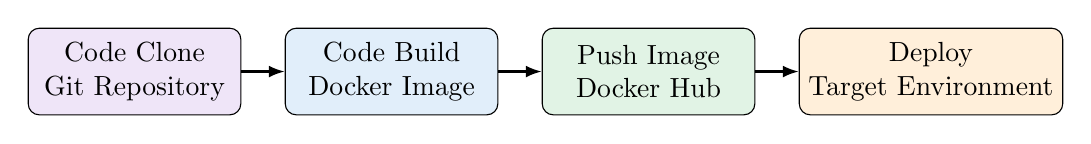
\begin{tikzpicture}[
 node distance=0.55cm,
 block/.style={draw,rounded corners,minimum width=2.7cm,minimum height=1.1cm,align=center,fill=lightpurple},
 arr/.style={-{Latex[length=2mm]},thick}
]
\node[block] (a) {Code Clone\\Git Repository};
\node[block,right=of a,fill=lightblue] (b) {Code Build\\Docker Image};
\node[block,right=of b,fill=lightgreen] (c) {Push Image\\Docker Hub};
\node[block,right=of c,fill=lightorange] (d) {Deploy\\Target Environment};
\draw[arr] (a)--(b); \draw[arr] (b)--(c); \draw[arr] (c)--(d);
\end{tikzpicture}
\caption{CI/CD pipeline stages described by Jenkinsfile}
\label{fig:jenkins}
\end{figure}

The pipeline depends on Jenkins being configured with the matching shared library, build agent, Docker access, Docker Hub credentials and deployment function. The presence of a Jenkinsfile documents the pipeline design; it does not by itself prove that the pipeline has been executed successfully.

\section{Testing and Quality Assurance}
Testing should be performed at multiple levels. Configuration checks confirm that Docker and Compose can parse the deployment files. Service checks confirm that containers start and remain running. Integration checks verify that Nginx can reach Django and Django can connect to MySQL. Functional checks verify the notes workflow from the browser.

\begin{table}[H]
\centering
\small
\begin{tabularx}{\textwidth}{|p{0.12\textwidth}|p{0.43\textwidth}|X|}
\hline
\textbf{Test ID} & \textbf{Test case} & \textbf{Expected outcome}\\ \hline
TC-01 & Build application image & Docker completes image build without dependency errors.\\ \hline
TC-02 & Start services with Compose & Nginx, Django and MySQL containers are created and started.\\ \hline
TC-03 & Check MySQL health & MySQL health check succeeds.\\ \hline
TC-04 & Check Django health endpoint & Configured endpoint returns a successful response.\\ \hline
TC-05 & Apply migrations & Django reports migrations completed or no pending migrations.\\ \hline
TC-06 & Open application in browser & Application responds at configured host endpoint.\\ \hline
TC-07 & Save a note & Note is stored successfully, if the operation is implemented in the UI.\\ \hline
TC-08 & Restart containers & Persisted database data remains available.\\ \hline
TC-09 & Inspect logs & Logs are available and show no critical startup failure.\\ \hline
TC-10 & Run Jenkins pipeline & Stages complete when required Jenkins configuration is present.\\ \hline
\end{tabularx}
\caption{Testing strategy and expected outcomes}
\label{tab:testing}
\end{table}

\section{Evaluation and Analysis}
The repository configuration demonstrates a containerized deployment design with separate Nginx, Django and MySQL services. The Django service is configured to run migrations and launch through Gunicorn. The database uses a mounted data directory, and health checks are defined for MySQL and Django. The Jenkinsfile documents a multi-stage pipeline for source retrieval, image building, image publishing and deployment.

The principal learning outcome is the integration of a Python web framework with container-based infrastructure. The project provides exposure to Docker images, containers, Compose services, networking, environment variables, persistent storage, reverse proxies and pipeline automation.

\section{Challenges and Limitations}
\begin{itemize}[leftmargin=0.4in]
\item The public README provides a concise setup guide but limited detailed documentation of user-facing workflows.
\item The visible Compose configuration contains example-style database credentials; these must be replaced before public or production deployment.
\item Service startup ordering and application readiness should be validated carefully.
\item The Jenkinsfile relies on a custom shared library, a labelled agent and configured credentials not contained in the repository.
\item The pipeline's source repository and deployment target should be confirmed before claiming successful execution.
\item Direct external access to the Django application port should be restricted in production.
\item Automated unit tests, load tests, backup tests and security scans should be added and reported only after execution.
\end{itemize}

% -------------------------------------------------
% CHAPTER 5
% -------------------------------------------------
\chapter{Experimental Result}

This chapter describes the results that can be assessed when the application is executed in the target environment. The repository configuration alone confirms the intended service arrangement, but screenshots and actual test outputs should be inserted after running the project. The following subsections provide the appropriate evidence locations and evaluation sequence.

\section{Application Startup and Service Status}
The application stack can be started using Docker Compose. The service status should be checked to confirm that the Nginx, Django and MySQL containers have been created and are running. A screenshot of the terminal output of \texttt{docker compose ps} can be inserted here.

\begin{figure}[H]
\centering
\fbox{\parbox[c][1.45in][c]{0.82\textwidth}{\centering Insert screenshot of successful Docker Compose service status here.}}
\caption{Docker Compose service status (insert actual screenshot)}
\label{fig:compose-result}
\end{figure}

\section{Browser Access}
The repository README indicates local application access at \url{http://localhost:8000}. The Compose file also publishes Nginx on host port 80. The actual URL depends on the active Nginx configuration and host port mappings. A screenshot of the running application in a browser should be inserted after verifying the correct endpoint.

\begin{figure}[H]
\centering
\fbox{\parbox[c][1.45in][c]{0.82\textwidth}{\centering Insert screenshot of the running Django Notes App here.}}
\caption{Django Notes App browser interface (insert actual screenshot)}
\label{fig:browser}
\end{figure}

\section{Notes Management Module}
The notes workflow should be tested using the operations available in the final user interface. For example, if the application provides note creation, editing, viewing and deletion, each operation should be tested with a valid input and its result recorded. Do not include a feature in the final report unless it is visible in the implementation.

\begin{figure}[H]
\centering
\fbox{\parbox[c][1.45in][c]{0.82\textwidth}{\centering Insert screenshot showing a note operation and its result here.}}
\caption{Notes management operation (insert actual screenshot)}
\label{fig:notes}
\end{figure}

\section{Database Persistence}
To verify persistence, create or update a record, restart the containers and check whether the record remains available. The MySQL data directory is mounted to host storage in the deployment configuration. A screenshot of the before-and-after verification can be inserted here.

\section{CI/CD Pipeline Result}
The Jenkinsfile defines source retrieval, image build, image push and deployment stages. Execution requires a configured Jenkins environment, shared library, agent and credentials. If the pipeline has been executed, insert a screenshot of the completed Jenkins build. Otherwise, report this section as a pipeline design rather than a successful execution.

\begin{figure}[H]
\centering
\fbox{\parbox[c][1.45in][c]{0.82\textwidth}{\centering Insert Jenkins pipeline screenshot here only if the pipeline was executed.}}
\caption{Jenkins pipeline execution (if available)}
\label{fig:jenkins-result}
\end{figure}

\section{Result Summary}
The expected deployment outcome is a browser-accessible Django application operating alongside a MySQL database and Nginx reverse proxy. The container configuration supports repeatable service startup, database persistence and health monitoring. The actual success of each test must be confirmed using the running application and recorded evidence.

% -------------------------------------------------
% CHAPTER 6
% -------------------------------------------------
\chapter{Technology Used}

\section{Frontend Technologies}
The browser interface is the presentation layer through which users interact with the notes application. The exact frontend templates, stylesheets and scripts should be identified from the project source. Django can render server-side HTML templates and serve static resources as configured.

\section{Backend Technologies}
Python is the programming language used by the Django application. Django provides URL routing, views, models, database migrations and other web-development facilities. The application is served through Gunicorn using the WSGI entry point configured in the project.

\section{Database Technology}
MySQL is a relational database management system. It stores structured records in tables and supports SQL queries. The project configures MySQL as a separate container and mounts its data directory to host storage for persistence.

\section{Containerization Technology}
Docker packages application code and dependencies into images and runs them as containers. Docker Compose defines the related services in one configuration file. In this project, Compose coordinates the Django application, MySQL database and Nginx web server.

\section{Web Server Technology}
Nginx is a web server and reverse proxy. It accepts browser requests and can forward them to an upstream application server. The project exposes the Nginx service on port 80. Gunicorn serves the Django WSGI application on port 8000 within the application service.

\section{Development and Automation Tools}
Git is a distributed version control system used to track source-code changes. GitHub hosts the project repository. Jenkins is an automation server commonly used for continuous integration and continuous delivery. The Jenkinsfile in the repository describes stages for cloning code, building a Docker image, pushing the image and deploying it.

% -------------------------------------------------
% CONCLUSION / FUTURE SCOPE / REFERENCES
% -------------------------------------------------
\chapter*{Conclusion}
\addcontentsline{toc}{chapter}{Conclusion}
The Django Notes App project demonstrates the development and containerized deployment of a Python-based web application. By combining Django with Docker and Docker Compose, the application environment is described through configuration files rather than relying entirely on manual host setup. The deployment design separates the web application, database and reverse-proxy responsibilities into distinct services.

The Dockerfile defines a Python 3.9-based application image, installs required dependencies and exposes the application port. Docker Compose coordinates Nginx, Django and MySQL, attaches them to a shared network, configures service dependencies and health checks, and mounts database storage for persistence. The Django service applies database migrations before launching Gunicorn. Nginx provides an HTTP entry point, while MySQL stores persistent application data.

The Jenkinsfile introduces the structure of a CI/CD pipeline through source cloning, Docker image building, image publishing and deployment stages. Its execution depends on Jenkins shared-library configuration, credentials and a deployment environment. Overall, the project provides a practical foundation for understanding web application deployment, containerization, reverse proxying, database persistence and DevOps automation.

\chapter*{Future Scope}
\addcontentsline{toc}{chapter}{Future Scope}
The project can be extended in several ways:
\begin{itemize}[leftmargin=0.4in]
\item Improve the notes editor with categories, tags, rich-text formatting, attachments and search.
\item Add or strengthen user authentication and ensure that each user can access only their own notes.
\item Introduce pagination, sorting, filtering and note archiving for larger collections.
\item Replace example credentials with Docker secrets or a secure secret-management service.
\item Use a dedicated least-privilege MySQL account instead of the root account for application access.
\item Restrict direct external access to the Django container and route public traffic only through Nginx.
\item Enable HTTPS using TLS certificates and configure secure cookies and security headers.
\item Add automated Django unit tests and integration tests to the CI pipeline.
\item Extend Jenkins with quality checks, vulnerability scanning, image tagging and rollback support.
\item Deploy the application to a cloud virtual machine or managed container platform.
\item Add monitoring, centralized logs, resource metrics and alerting.
\item Implement scheduled database backups and periodically test data restoration.
\end{itemize}

\chapter*{References}
\addcontentsline{toc}{chapter}{References}
\begin{enumerate}[label={[\arabic*]},leftmargin=0.45in]
\item Govind Kotalwar, ``Django Notes App,'' GitHub repository. [Online]. Available: \url{https://github.com/govindkotalwar8/django-notes-app}
\item Django Software Foundation, ``Django Documentation.'' [Online]. Available: \url{https://docs.djangoproject.com/}
\item Docker, ``Docker Documentation.'' [Online]. Available: \url{https://docs.docker.com/}
\item Docker, ``Docker Compose Documentation.'' [Online]. Available: \url{https://docs.docker.com/compose/}
\item MySQL, ``MySQL Reference Manual.'' [Online]. Available: \url{https://dev.mysql.com/doc/}
\item Nginx, ``Nginx Documentation.'' [Online]. Available: \url{https://nginx.org/en/docs/}
\item Gunicorn, ``Gunicorn Documentation.'' [Online]. Available: \url{https://docs.gunicorn.org/}
\item Jenkins, ``Jenkins User Documentation.'' [Online]. Available: \url{https://www.jenkins.io/doc/}
\item Python Software Foundation, ``Python 3 Documentation.'' [Online]. Available: \url{https://docs.python.org/3/}
\end{enumerate}

\appendix
\chapter{Important Commands}
\begin{longtable}{|p{0.48\textwidth}|p{0.42\textwidth}|}
\hline
\textbf{Command} & \textbf{Purpose}\\ \hline
\texttt{docker --version} & Check Docker installation.\\ \hline
\texttt{docker compose version} & Check Docker Compose installation.\\ \hline
\texttt{docker compose up --build} & Build images and start services.\\ \hline
\texttt{docker compose up -d} & Start services in detached mode.\\ \hline
\texttt{docker compose ps} & Display service/container status.\\ \hline
\texttt{docker compose logs -f} & Follow logs from all services.\\ \hline
\texttt{docker compose build --no-cache} & Rebuild images without build cache.\\ \hline
\texttt{docker compose down} & Stop and remove containers and network.\\ \hline
\texttt{docker exec -it django\_cont python manage.py migrate} & Run Django migrations inside the application container.\\ \hline
\caption{Important Docker and Django commands}
\end{longtable}

\chapter{Repository Details}
The project repository supplied for this report is available at:

\url{https://github.com/govindkotalwar8/django-notes-app}

The repository URL above is retained exactly as supplied. If the project has been transferred to a different GitHub owner or renamed, replace this URL with the confirmed repository address before submission.

\end{document}
